\chapter{Rekursion}
\renewcommand{\chaptertitle}{Rekursion}

\lehead[]{\normalfont\sffamily\hspace*{-2.00cm}\textcolor{white}{\colorbox{lightblue}{\makebox[1.60cm][r]{\thechapter}}}\hspace{0.17cm}\textcolor{lightblue}{\chaptertitle}}
\rohead[]{\textcolor{lightblue}{\chaptertitle}\normalfont\sffamily\hspace*{0.17cm}\textcolor{white}{\colorbox{lightblue}{\makebox[1.60cm][l]{\thechapter}}}\hspace{-2.00cm}}
%\chead[]{}
\rehead[]{\textcolor{lightblue}{AvHG, Inf, My}}
\lohead[]{\textcolor{lightblue}{AvHG, Inf, My}}

\lstset{style=myJava}

\section{Rekursions-Begriff}

Rekursion bedeutet, dass auf etwas Bekanntes zurückgegriffen wird. In der
Programmierung tritt eine Rekursion auf, wenn eine Funktion in ihrem Code auf
sich selber zurückgreift.

\subsection{Blick in den Spiegel}

Wenn man den Bildschirminhalt filmt (Screen-Capturing) und das Ergebnis am
Bildschirm betrachtet, dann erhält man einen rekursiven Effekt:

\begin{minipage}{1.0\textwidth}
  \centering
  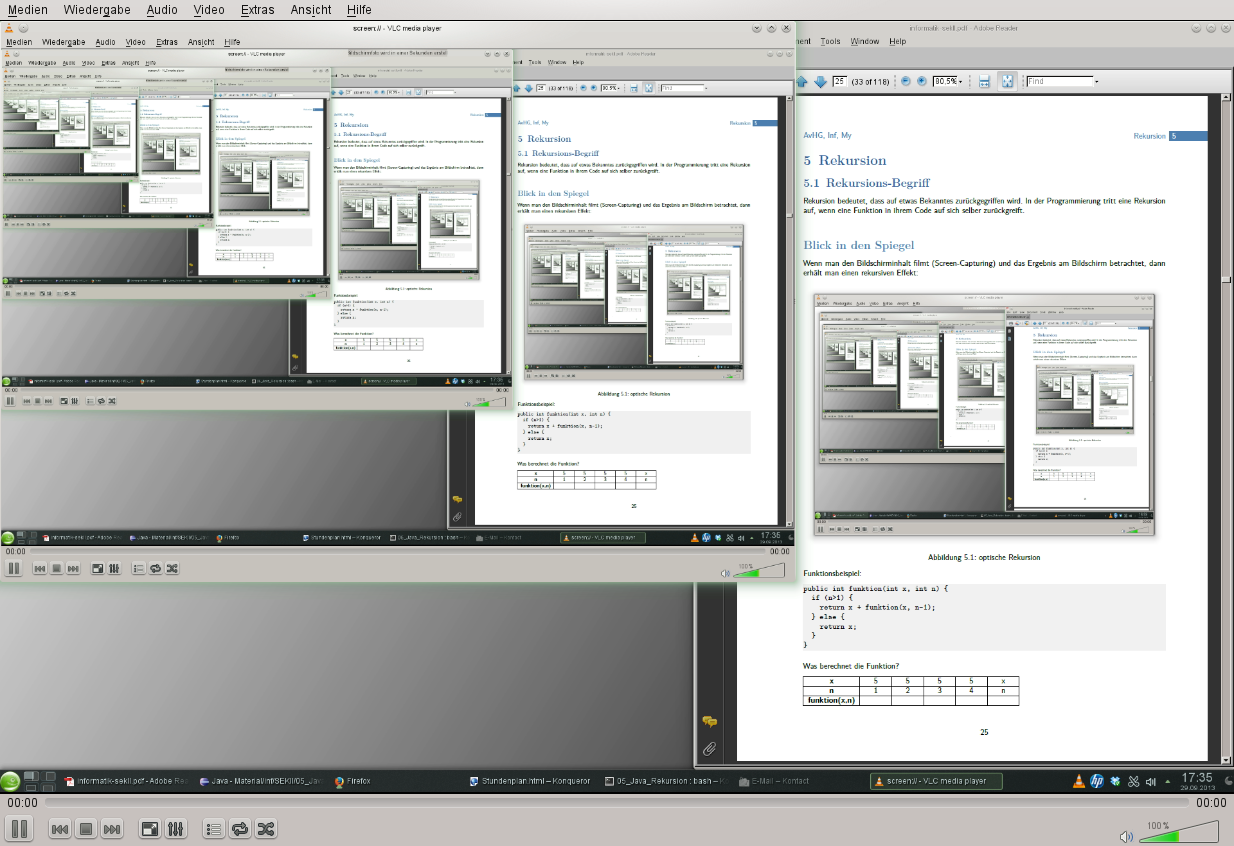
\includegraphics[width=1.0\textwidth]{./inf/SEKII/06_Java_Rekursion/rekursiverDesktop.png}
  \captionof{figure}{optische Rekursion}
\end{minipage}

%Es war einmal ein Mann,\\
%\hspace*{0.5cm} der einen Mann sah (2),\\
%\hspace*{1.0cm}	der einen Mann sah (1),\\
%\hspace*{1.5cm}		der einen Mann sah (0),\\
%\hspace*{1.5cm}		der sich rasierte (0),\\
%\hspace*{1.0cm}	der sich rasierte (1),\\
%\hspace*{0.5cm} der sich rasierte (2),\\
%der sich rasierte. 


Funktionsbeispiel:

\begin{lstlisting}
public int funktion(int x, int n) {
  if (n>1) {
    return x + funktion(x, n-1);
  } else {
    return x;
  }
}
\end{lstlisting}

Was berechnet die Funktion?

\begin{tabular}{|c|c|c|c|c|c|}\hline
\textbf{x}             & 5 & 5 & 5 & 5 & x \\ \hline
\textbf{n}             & 1 & 2 & 3 & 4 & n \\ \hline
\textbf{funktion(x,n)} &  \hspace{1cm} & \hspace{1cm} & \hspace{1cm} &
\hspace{1cm} & \hspace{1cm} \\
\hline
\end{tabular}


\subsection{Rekursiv Programmieren}

Nicht alle Probleme lassen sich rekursiv lösen. Aber es gibt eine Reihe von
Problemen, die sich entweder nur rekursiv lösen lassen, oder die sich zumindest
mit Hilfe eines rekursiven Ansatzes sehr viel eleganter lösen lassen als ohne.

Wenn du den rekursiven Ansatz wählst, musst du folgende beiden Fragen
beantworten:

\begin{compactenum}[1.]
\item Für welchen Parameter-Wert ist die Lösung bekannt? Am Beispiel der
Fakultät: Die Fakultät von 0 ist definiert als 1.
\item Wie lässt sich das Ergebnis für alle anderen Parameter-Werte berechnen,
wenn man annimmt, dass das Ergebnis für den um 1 verringerten Parameter-Wert
bereits bekannt ist?
\end{compactenum}

Um die Fakultät einer gegebenen positiven ganzen Zahl zu berechnen ruft die
rekursiv programmierte Methode \lstinline|fakultaet()| sich immer wieder mit
einem jeweils um 1 verringerten Parameter-Wert auf. Dabei warten die zuerst
aufgerufenen Methoden \lstinline|fakultaet()| solange auf die Ergebnisse ihrer
\glqq Kinder\grqq\ bis der Parameter-Wert auf diese Weise den Wert 0 erreicht
hat. Sobald das passiert ist ein konkretes Ergebnis bekannt. Zunächst nur das
Ergebnis des \glqq jüngsten Kindes\grqq , dann des zweitjüngsten usw. Bis
schließlich die zuerst aufgerufene \lstinline|fakultaet()|-Methode von seinem
Kind das Ergebnis geliefert bekommt und damit in die Lage versetzt wird, das
endgültige Ergebnis zu berechnen.

Schau dir dazu noch mal das Programm-Beispiel auf der vorherigen Seite an.

